\documentclass[12pt, titlepage]{article}

\usepackage[margin=1in]{geometry}
\usepackage[hidelinks]{hyperref}
\usepackage{amsmath}
\usepackage{float}
\usepackage{graphicx}
% \usepackage{newtxtext}  % WHY IS THIS HERE
\usepackage{listings}
\usepackage{circuitikz}
\usepackage{color}
\usepackage{multicol}


% Define colors
\definecolor{deepblue}{rgb}{0,0,0.5}
\definecolor{deepred}{rgb}{0.6,0,0}
\definecolor{deepgreen}{rgb}{0,0.5,0}


% Python style for highlighting
\newcommand\pythonstyle{\lstset{
    language=Python,
    basicstyle=\ttm,
    otherkeywords={self},             % Add keywords here
    keywordstyle=\ttb\color{deepblue},
    emph={bin,_prod,__name__},          % Custom highlighting
    emphstyle=\ttb\color{deepred},    % Custom highlighting style
    stringstyle=\color{deepgreen},
    commentstyle=\color{deepgreen},
    frame=tb,
    % Any extra options here
    showstringspaces=false
}}
\newcommand\pythonexternal[2][]{{\pythonstyle\lstinputlisting[#1]{#2}}}
\newcommand\bbar[1]{\mathop{\overline{#1 \vphantom A}}}
\newcommand\sA{\ensuremath{\mathtt{A}}}
\newcommand\sB{\ensuremath{\mathtt{B}}}
\newcommand\Aa{\ensuremath{\mathtt{A_0}}}
\newcommand\Ab{\ensuremath{\mathtt{A_1}}}
\newcommand\Ba{\ensuremath{\mathtt{B_0}}}
\newcommand\Bb{\ensuremath{\mathtt{B_1}}}
\newcommand\Qa{\ensuremath{\mathtt{Q_0}}}
\newcommand\Qb{\ensuremath{\mathtt{Q_1}}}
\newcommand\Ca{\ensuremath{\mathtt{C_0}}}
\newcommand\us{$\mathrm{\mu}$s}

% Author information
\title{ENCM 467 Lab 4\\Building Digital Logic Systems}
\author
{
    William Doan\\
    Taras Kuzyk\\
    Andreas Smit
}
\date{December 7, 2020}


% Settings
\setlength{\parindent}{0pt}

\begin{document}
    \maketitle

    \section{CMOS Digital Logic Gates}\label{sec:gates}
    There are 4 digital logic gates that will be used throughout this
    lab, a CMOS NAND gate (figure \ref{fig:NAND}), a CMOS NOR gate
    (figure \ref{fig:NOR}), a CMOS XOR gate (figure \ref{fig:XOR})
    and a CMOS NOT gate (figure \ref{fig:NOT}).
    \begin{multicols}{2}
        \begin{figure}[H]
            \centering
            \begin{circuitikz}
                \draw (-1, 5) node[pmos](QPA){}
                (QPA.G)node[left]{$\mathtt{A}$};
                \draw (1, 5) node[pmos, xscale=-1](QPB){}
                (QPB.G)node[right]{$\mathtt{B}$};
                \draw (0, 3) node[nmos](QNB){}
                (QNB.G)node[left]{$\mathtt{B}$};
                \draw (0, 1) node[nmos](QNA){}
                (QNA.G)node[left]{$\mathtt{A}$};
                \draw (QPA.S) node[vcc]{$V_{DD}$} (QPB.S)
                node[vcc]{$V_{DD}$};
                \draw (QPA.D) to (-1, 4) to (1, 4) to (QPB.D) (1, 4) to
                (1.5, 4) node[right]{$V_{out} = \bbar{\sA\sB}$};
                \draw (0, 4) to (QNB.D);
                \draw (QNB.S) to (QNA.D);
                \draw (QNA.S) node[vee]{$V_{SS}$};
            \end{circuitikz}
            \caption{A CMOS NAND Gate}
            \label{fig:NAND}
        \end{figure}
        \begin{figure}[H]
            \centering
            \begin{circuitikz}
                \draw (0, 5) node[pmos](QPA){}
                (QPA.G)node[left]{$\mathtt{A}$};
                \draw (0, 3) node[pmos](QPB){}
                (QPB.G)node[left]{$\mathtt{B}$};
                \draw (1, 1) node[nmos, xscale=-1](QNB){}
                (QNB.G)node[right]{$\mathtt{B}$};
                \draw (-1, 1) node[nmos](QNA){}
                (QNA.G)node[left]{$\mathtt{A}$};
                \draw (QPA.S) node[vcc]{$V_{DD}$};
                \draw (QPA.D) to (QPB.S);
                \draw (QPB.D) to (0, 2) (QNA.D) to (-1, 2) to (1, 2) to
                (QNB.D) (1, 2) to (1.5, 2)
                node[right]{$V_{out} = \bbar{\sA + \sB}$};
                \draw (QNA.S) node[vee]{$V_{SS}$} (QNB.S)
                node[vee]{$V_{SS}$};
            \end{circuitikz}
            \caption{A CMOS NOR Gate}
            \label{fig:NOR}
        \end{figure}
        \begin{figure}[H]
            \centering
            \begin{circuitikz}
                \draw (-1, 7) node[pmos](Q1){}
                (Q1.G)node[left]{$\sB$};
                \draw (1, 7) node[pmos, xscale=-1](Q2){}
                (Q2.G)node[right]{$\sA$};
                \draw (-1, 5) node[pmos](Q3){}
                (Q3.G)node[left]{$\bbar\sB$};
                \draw (1, 5) node[pmos, xscale=-1](Q4){}
                (Q4.G)node[right]{$\bbar\sA$};
                \draw (4, 7) node[pmos, scale=0.5](Q5){};
                \draw (4, 2) node[pmos, scale=0.5](Q6){};
                \draw (-1, 3) node[nmos](Q7){}
                (Q7.G)node[left]{$\sA$};
                \draw (1, 3) node[nmos, xscale=-1](Q8){}
                (Q8.G)node[right]{$\bbar\sA$};
                \draw (-1, 1) node[nmos](Q9){}
                (Q9.G)node[left]{$\sB$};
                \draw (1, 1) node[nmos, xscale=-1](Q10){}
                (Q10.G)node[right]{$\bbar\sB$};
                \draw (4, 6) node[nmos, scale=0.5](Q11){};
                \draw (4, 1) node[nmos, scale=0.5](Q12){};
                \draw (Q1.S) node[vcc]{$V_{DD}$}
                (Q2.S)node[vcc]{$V_{DD}$}
                (Q5.S)node[vcc, scale=0.5]{$V_{DD}$}
                (Q6.S)node[vcc, scale=0.5]{$V_{DD}$};
                \draw (Q9.S) node[vee]{$V_{SS}$}
                (Q10.S)node[vee]{$V_{SS}$}
                (Q11.S)node[vee, scale=0.5]{$V_{SS}$}
                (Q12.S)node[vee, scale=0.5]{$V_{SS}$};
                \draw (Q1.D) to (Q2.D) to (Q4.S) (Q1.D) to (Q3.S);
                \draw (Q3.D) to (Q4.D) to (Q8.D) (Q3.D) to (Q7.D)
                (1, 4) to (1.5, 4)node[right](){$V_{out}=\sA\oplus\sB$};
                \draw (Q7.S) to (Q9.D) (Q8.S) to (Q10.D);
                \draw (3, 1.5) node[left](){$\sB$} to (3.5, 1.5) to
                (3.5, 2) to (Q6.G) (3.5, 1.5) to (3.5, 1) to (Q12.G);
                \draw (Q6.D) to (Q12.D) (4, 1.5) to (4.5, 1.5)
                node[right](){$\bbar\sB$};
                \draw (3, 6.5) node[left](){$\sA$} to (3.5, 6.5) to
                (3.5, 7) to (Q5.G) (3.5, 6.5) to (3.5, 6) to (Q11.G);
                \draw (Q5.D) to (Q11.D) (4, 6.5) to (4.5, 6.5)
                node[right](){$\bbar\sA$};
            \end{circuitikz}
            \caption{A CMOS XOR Gate}
            \label{fig:XOR}
        \end{figure}
        \begin{figure}[H]
            \centering
            \begin{circuitikz}
                \draw (0, 3) node[pmos](QP){};
                \draw (0, 1) node[nmos](QN){};
                \draw (QP.S) node[vcc]{$V_{DD}$};
                \draw (QN.S) node[vee]{$V_{SS}$};
                \draw (QP.D) to (QN.S) (0, 2) to (0.5, 2)
                node[right](){$V_{out} = \bbar\sA$};
                \draw (-1.5, 2) node[left](){$\sA$} to (-1, 2) to
                (-1, 3) to (QP.G) (-1, 2) to (-1, 1) to (QN.G);
            \end{circuitikz}
            \caption{A CMOS NOT Gate}
            \label{fig:NOT}
        \end{figure}
    \end{multicols}
    The NAND, NOR, XOR, and NOT gates are implemented in LTspice using
    the CD 4007 CMOS integrated circuit as shown in figures
    \ref{fig:NAND_lt}, \ref{fig:NOR_lt}, \ref{fig:XOR_lt}, and
    \ref{fig:NOT_lt} respectively. All inputs not used are tied to
    ground to prevent floating inputs.
    \begin{multicols}{2}
        \begin{figure}[H]
            \centering
            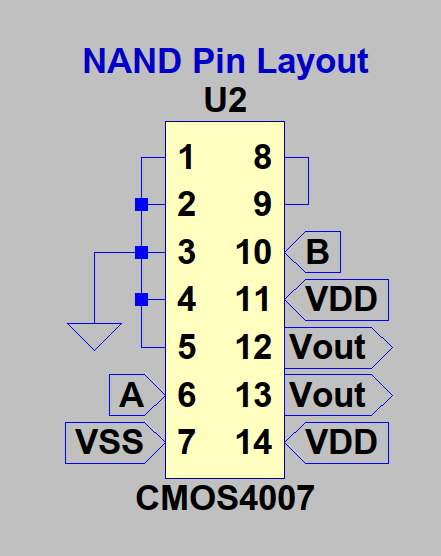
\includegraphics[width=0.6\linewidth]{figures/NAND_circuit.png}
            \caption{The NAND circuit built in LTspice.}
            \label{fig:NAND_lt}
        \end{figure}
        \begin{figure}[H]
            \centering
            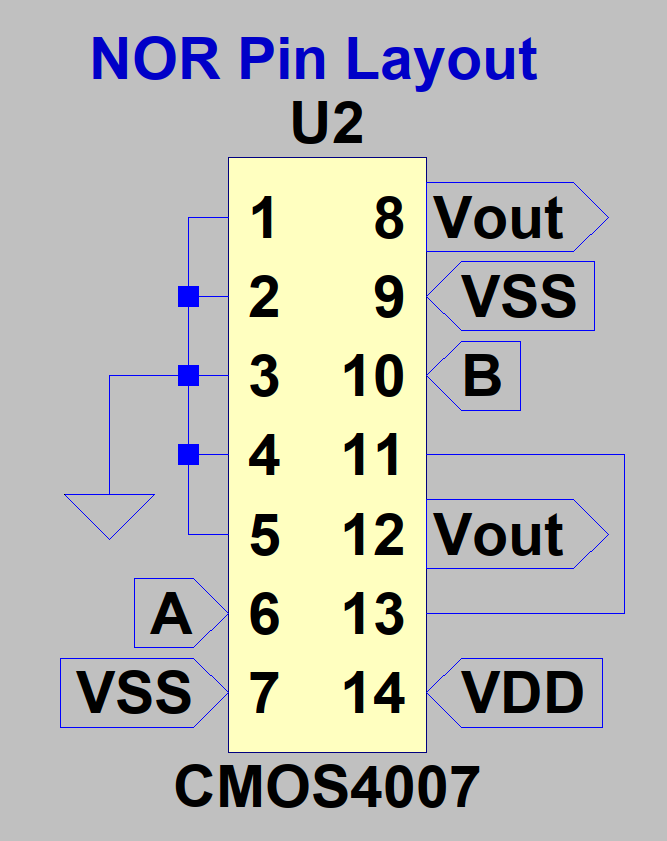
\includegraphics[width=0.6\linewidth]{figures/NOR_circuit.png}
            \caption{The NOR circuit built in LTspice.}
            \label{fig:NOR_lt}
        \end{figure}
        \begin{figure}[H]
            \centering
            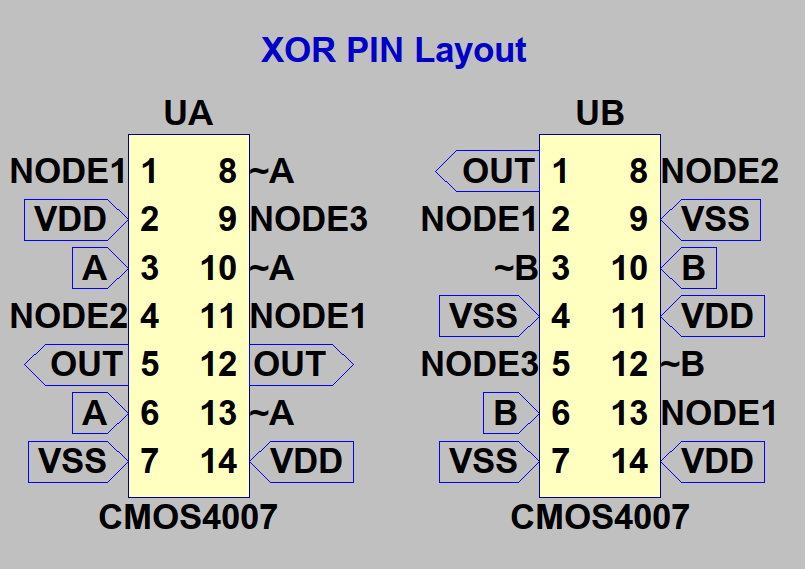
\includegraphics[width=0.6\linewidth]{figures/XOR_circuit.png}
            \caption{The XOR circuit built in LTspice.}
            \label{fig:XOR_lt}
        \end{figure}
        \begin{figure}[H]
            \centering
            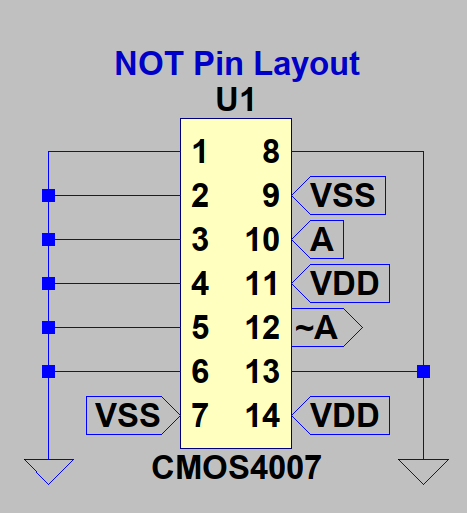
\includegraphics[width=0.6\linewidth]{figures/NOT_circuit.png}
            \caption{The NOT circuit built in LTspice.}
            \label{fig:NOT_lt}
        \end{figure}
    \end{multicols}
    The NAND, NOR, XOR, and NOT circuits are then exported as a sub
    circuit similar to the CMOS4007 component so that they can be reused
    throughout the rest of the lab as a discrete component.

    \section{Two Bit Adder}
    A two bit adder circuit is built using the components defined in
    section \ref{sec:gates} using LTspice (shown in figure
    \ref{fig:adder}.
    \begin{figure}[H]
        \centering
        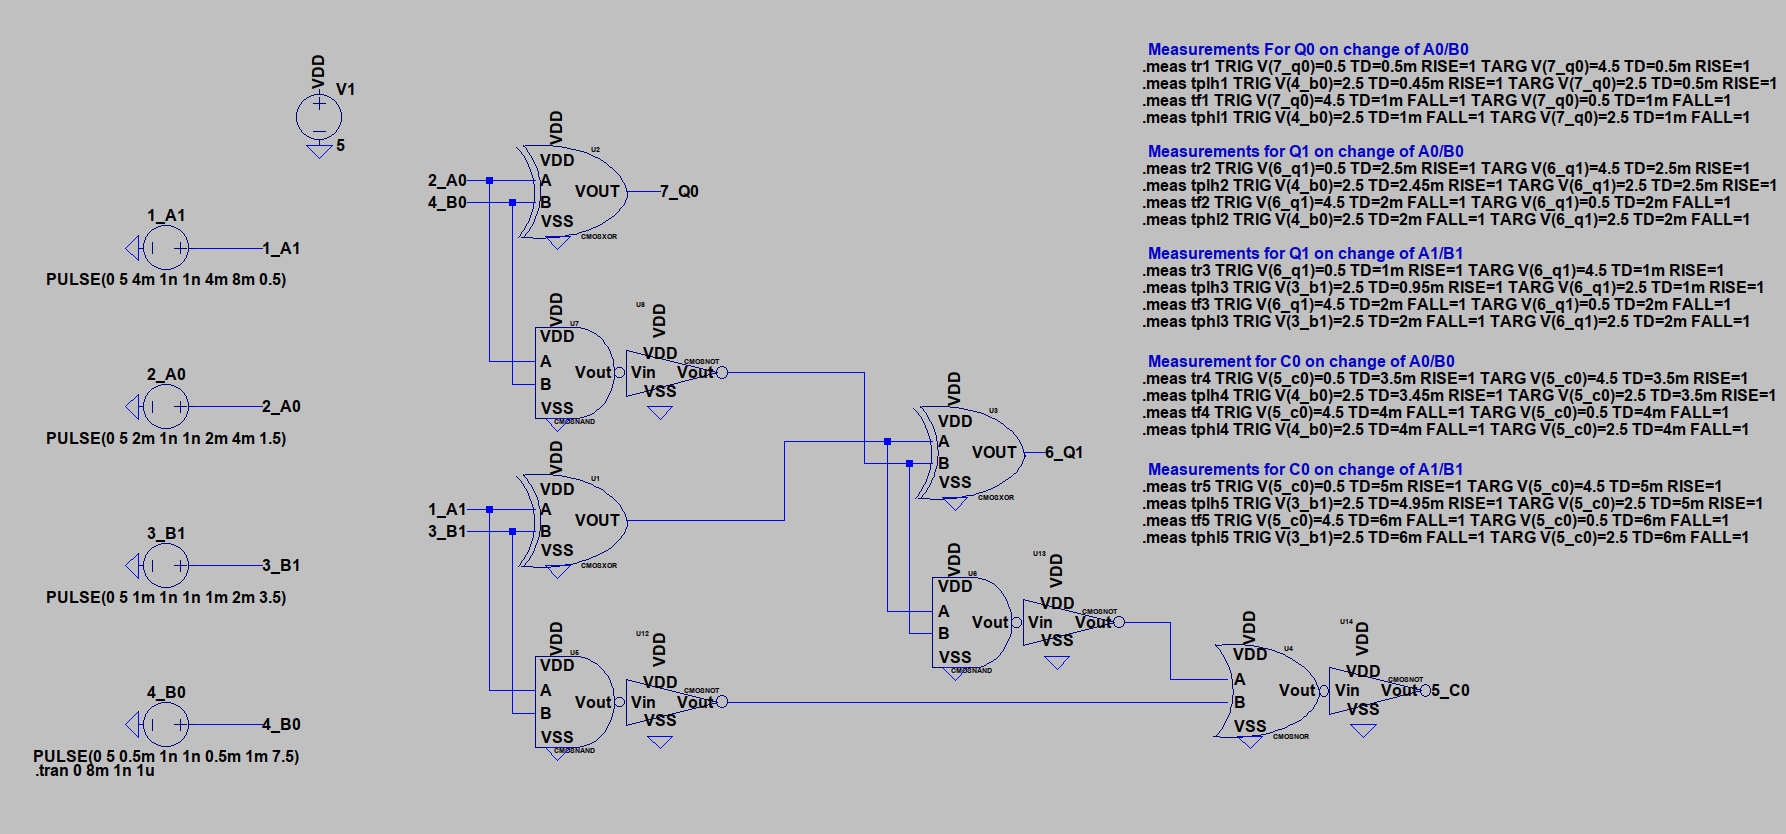
\includegraphics[width=0.9\textwidth]{figures/circuit.png}
        \caption{The 2-bit full adder built in LTspice.}
        \label{fig:adder}
    \end{figure}

    \subsection{Timing Diagram}
    The outputs are then measured over the course of 8ms as the inputs
    are stimulated. The outputs and inputs are shown in the timing
    diagram in figure \ref{fig:timing}.
    \begin{figure}[H]
        \centering
        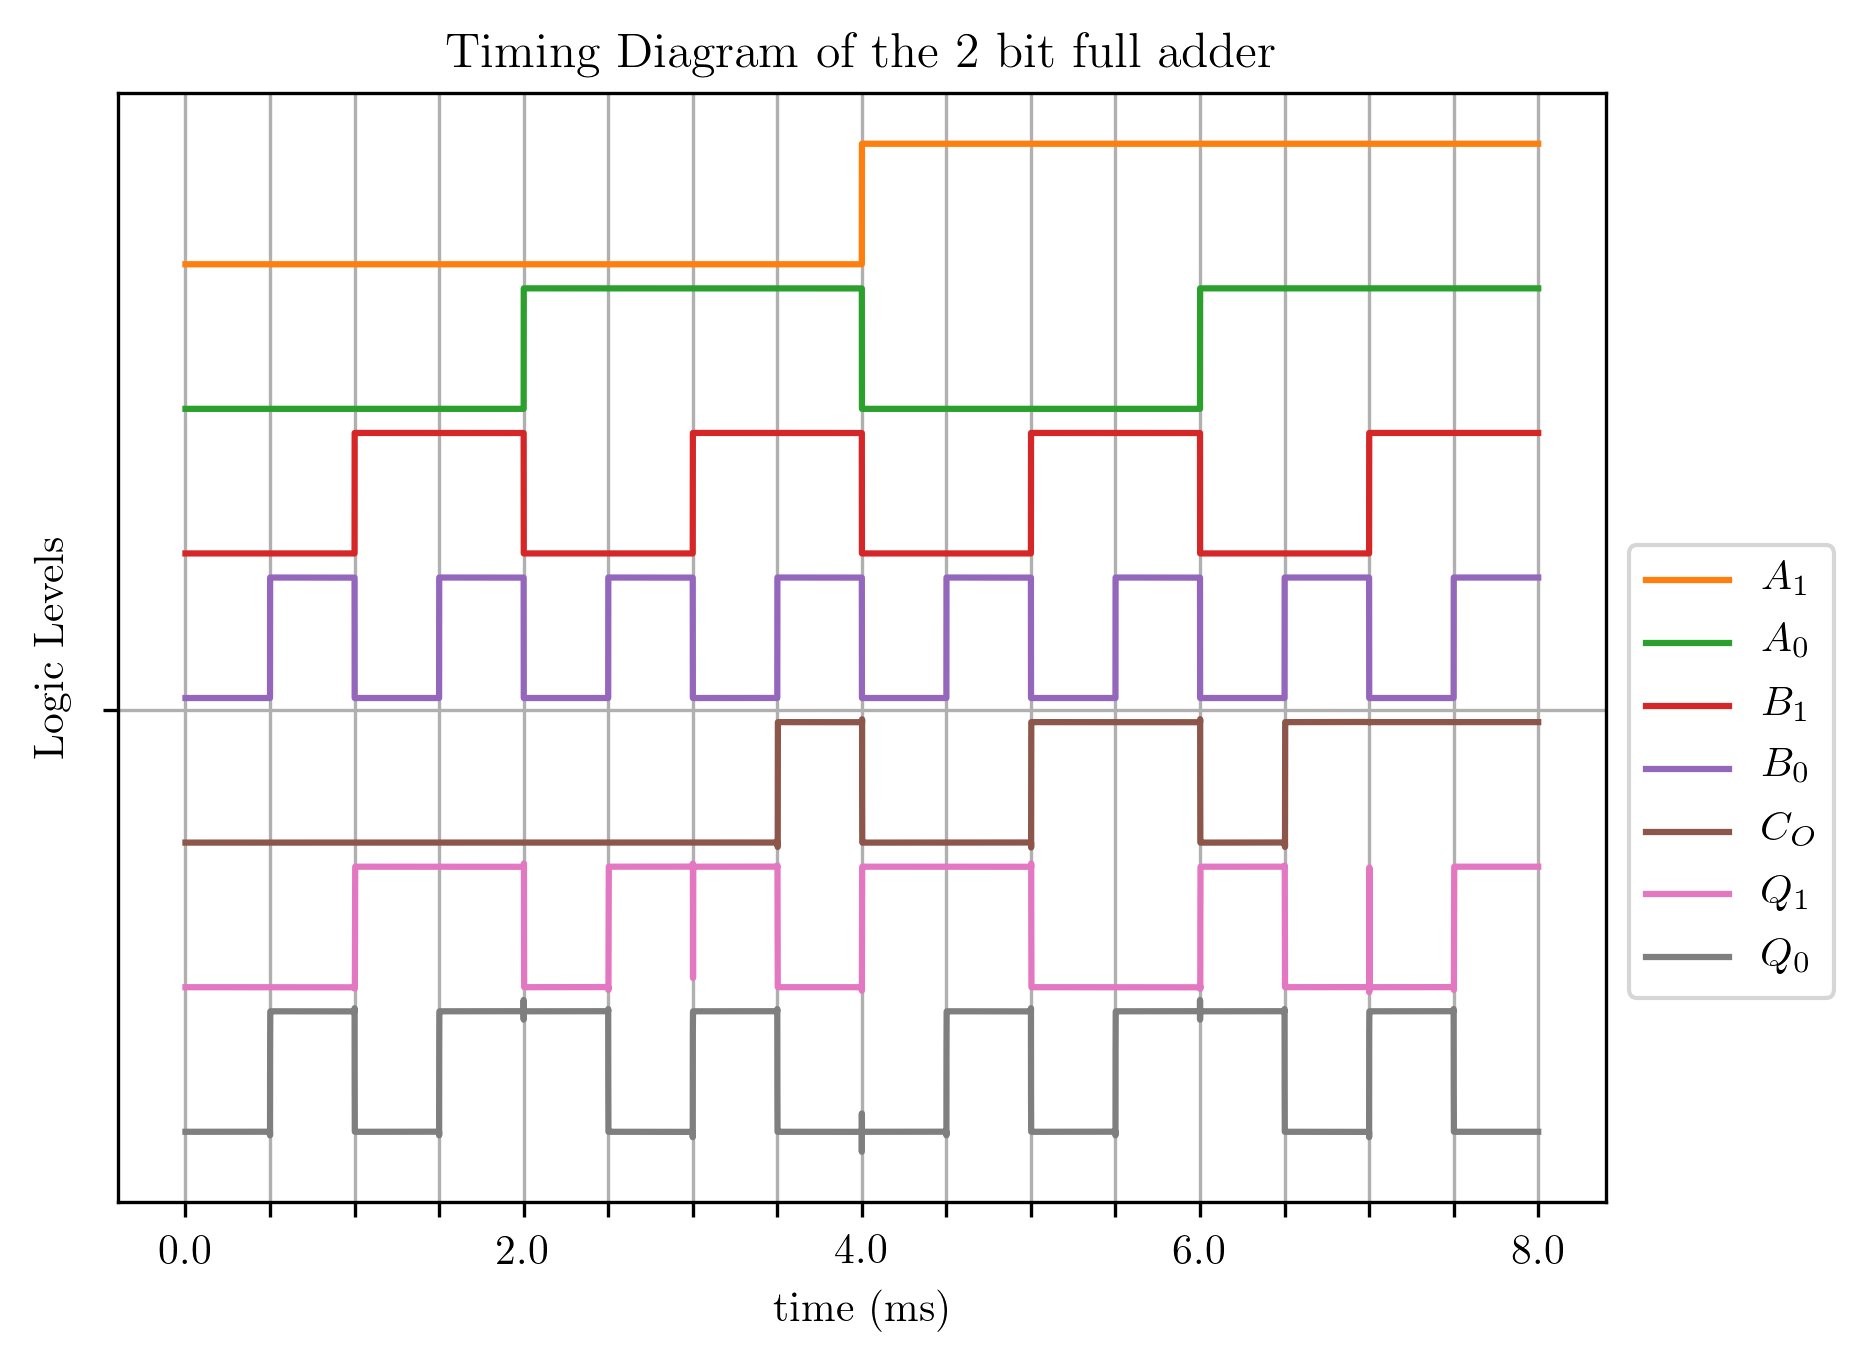
\includegraphics[width=0.9\textwidth]{figures/timing.png}
        \caption{The timing diagram of the 2-bit full adder}
        \label{fig:timing}
    \end{figure}
    In the timing diagram above a high logic level is when the signal is
    at 5V and a low logic level is when the signal is at 0V. We can see
    a few glitches in the logic gate due to the timing effects from
    different inputs. For example at 7ms $\Bb$ goes high and $\Ba$ goes
    low; When the transition at 7ms occurs, $\Qb$ briefly starts to go
    high. This happens as the gate responds first to $\Bb$ going high
    causing $\Qb$ to begin to raise, but then the gate responds to $\Ba$
    going low causing $\Qb$ to go low again.\\

    \subsection{Truth Table}
    The stable input and output values from the timing diagram in figure
    \ref{fig:timing} are placed into the truth table, table
    \ref{fig:truth}.
    \begin{table}[H]
        \centering
        \caption{The truth table for the 2-bit full adder}
        \label{fig:truth}
        \begin{tabular}{cc|cc||ccc}
            $\Ab$ & $\Aa$ & $\Bb$ & $\Ba$ & $\Ca$ & $\Qb$ & $\Qa$\\
            \hline
            0 & 0 & 0 & 0 & 0 & 0 & 0\\
            0 & 0 & 0 & 1 & 0 & 0 & 1\\
            0 & 0 & 1 & 0 & 0 & 1 & 0\\
            0 & 0 & 1 & 1 & 0 & 1 & 1\\
            0 & 1 & 0 & 0 & 0 & 0 & 1\\
            0 & 1 & 0 & 1 & 0 & 1 & 0\\
            0 & 1 & 1 & 0 & 0 & 1 & 1\\
            0 & 1 & 1 & 1 & 1 & 0 & 0\\
            1 & 0 & 0 & 0 & 0 & 1 & 0\\
            1 & 0 & 0 & 1 & 0 & 1 & 1\\
            1 & 0 & 1 & 0 & 1 & 0 & 0\\
            1 & 0 & 1 & 1 & 1 & 0 & 0\\
            1 & 1 & 0 & 0 & 0 & 1 & 1\\
            1 & 1 & 0 & 1 & 1 & 0 & 0\\
            1 & 1 & 1 & 0 & 1 & 0 & 1\\
            1 & 1 & 1 & 1 & 1 & 1 & 0\\
        \end{tabular}
    \end{table}

    \subsection{Timing Values}
    Finally the timing values are measured using the measure statements
    in the circuit shown in figure \ref{fig:adder} and are given in
    table \ref{tab:timings}.
    \begin{table}[H]
        \centering
        \caption{Timing values for the 2-bit full adder.}
        \label{tab:timings}
        \begin{tabular}{c|c|c|c|c|c}
            Case & Change in $\Qa$ & Change in $\Qb$ & Change in $\Qb$ &
            Change in $\Ca$ & Change in $\Ca$\\
            & due to $\Aa/\Ba$ & due to $\Aa/\Ba$ & due to $\Ab/\Bb$ &
            due to $\Aa/\Ba$ & due to $\Ab/\Bb$\\
            \hline
            $\tau_{PLH} $ & 546ns & 1.837\us & 2.184\us & 2.184\us &
            1.344\us\\
            $\tau_{PHL} $ & 596ns & 2.216\us & 2.216\us & 1.791\us &
            1.175\us\\
            $t_s$      & 571ns & 2.027\us & 2.200\us & 1.988\us &
            1.260\us\\
            $t_{rise}$ & 612ns & 629ns & 610ns & 175ns & 169ns\\
            $t_{fall}$ & 525ns & 544ns & 544ns & 248ns & 251ns
        \end{tabular}
    \end{table}
    As we can see in table \ref{fig:timing} the propagation delay is
    generally much longer than the rise and fall time for the 2-bit full
    adder. This is because the signal takes longer for it to propagate
    through the gate then it does for the output to fall. For example
    for the output $\Ca$ to respond to a change in $\Aa$ or $\Ba$ the
    signal from $\Aa$ or $\Ba$ has to travel through 2 NAND gates, a NOR
    gate and 3 NOT Gates. This takes a significant amount of time.
    However when the signal reaches the final not gate, the gate takes
    only a few nanoseconds to rise or fall accordingly causing the
    rising and falling of the signals to be much faster than the
    propagation times.\\

    This effect can clearly be seen in the graph in figure
    \ref{fig:delay}.
    \begin{figure}[H]
        \centering
        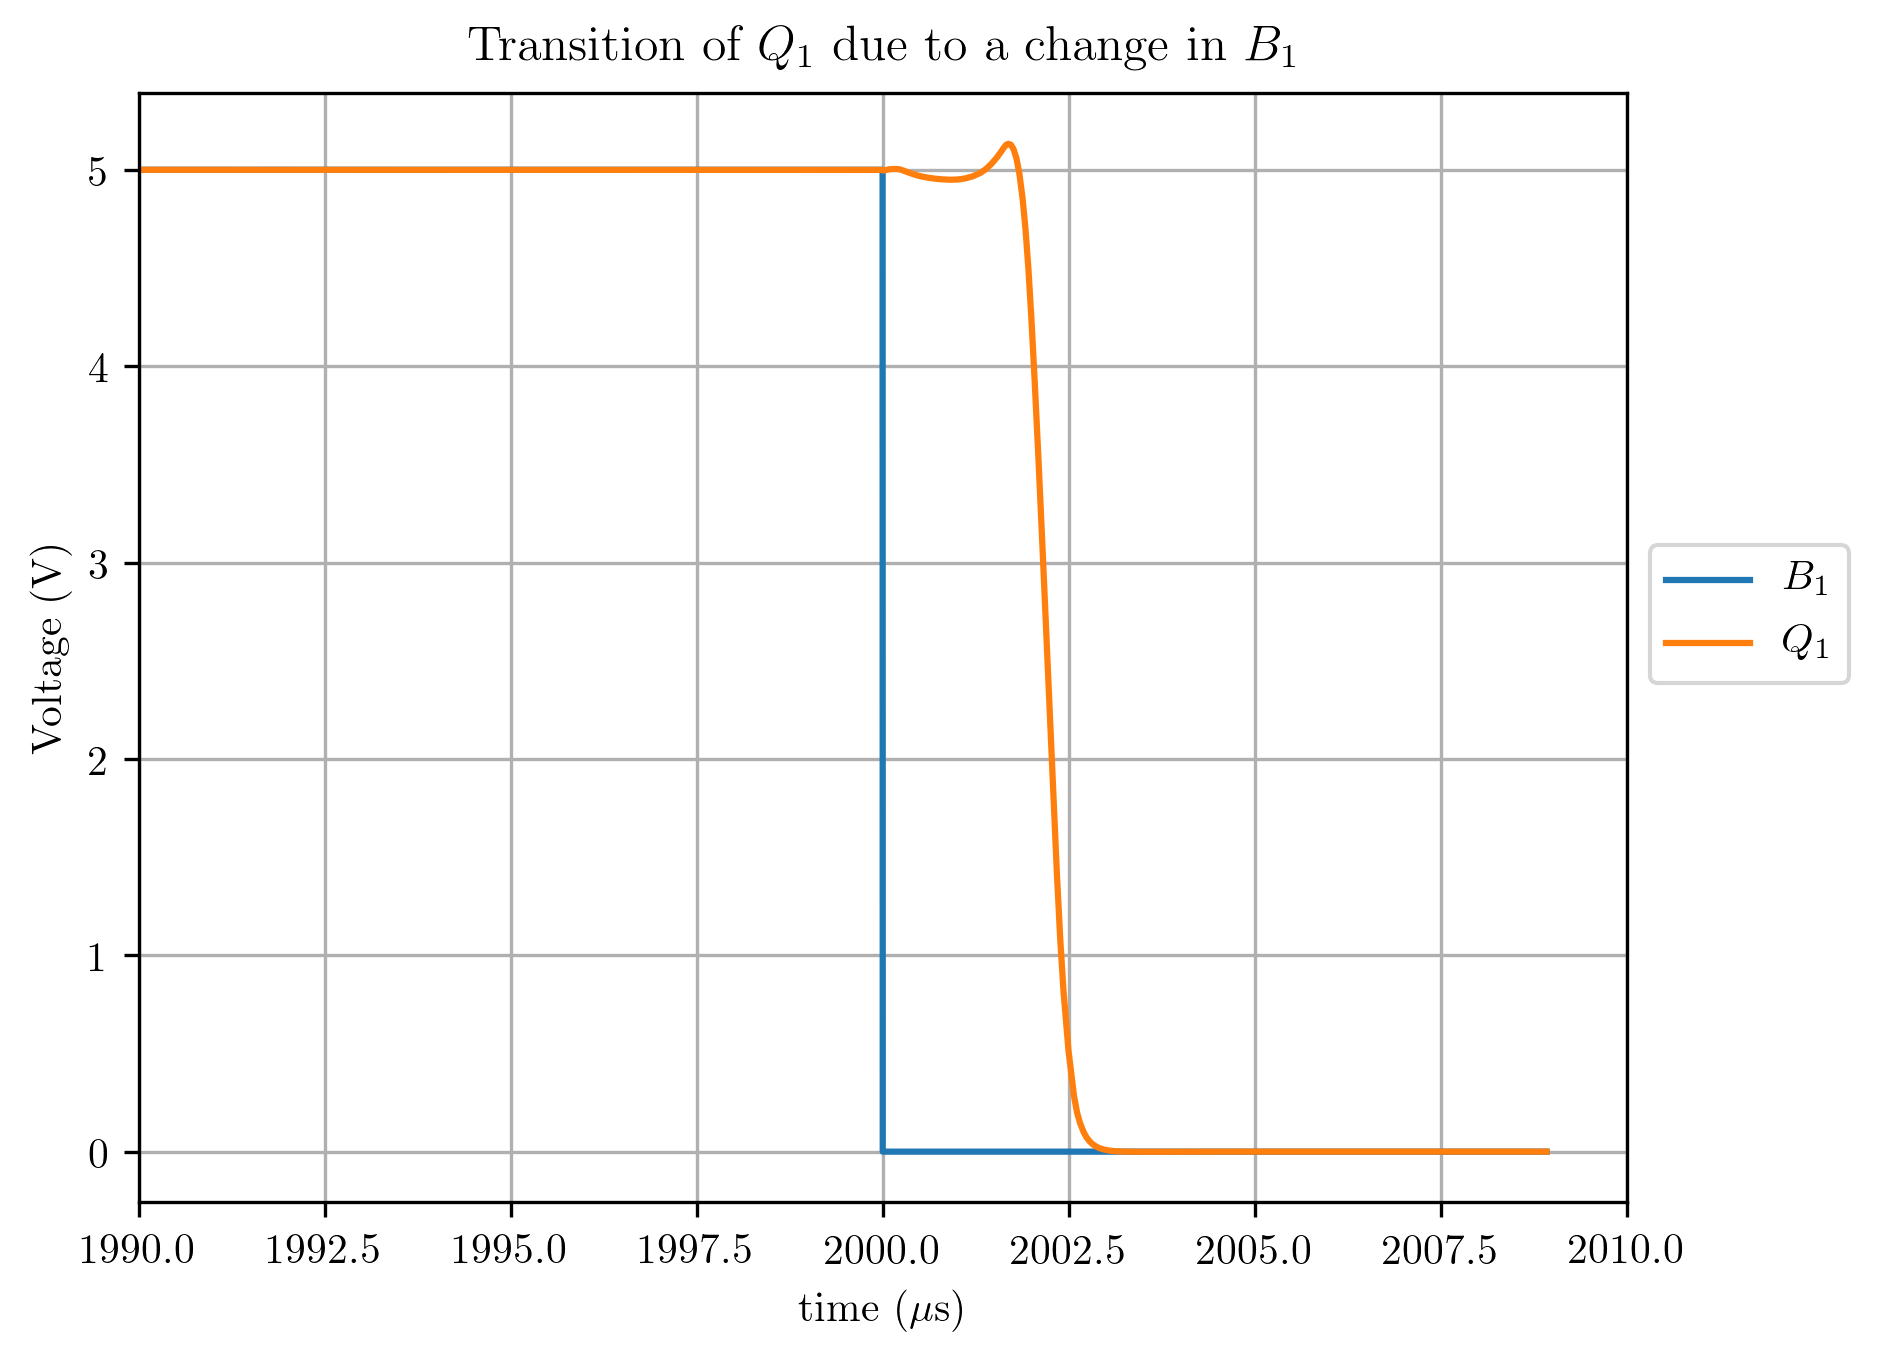
\includegraphics[width=0.7\textwidth]{figures/delays.png}
        \caption{The delay in the output $\Qb$ due to a change in $\Bb$
        is clearly present in this graph.}
        \label{fig:delay}
    \end{figure}
    The output $\Qb$ doesn't begin to fall due to the input $\Bb$ for
    almost 1.5\us{} after $\Bb$ falls. But when $\Qb$ starts to fall it
    falls to 0V in around than 0.5\us. The graph also verifies the data
    for the fall times of $\Qb$ from $\Bb$ in table \ref{tab:timings}.
    If we were to look at the rest of the transitions we would see a
    similar effect where the gate changes with a quick rise or fall time
    after a longer propagation delay.


\end{document}
